\documentclass[11pt,a4paper,]{article}
\usepackage{lmodern}

\usepackage{amssymb,amsmath}
\usepackage{ifxetex,ifluatex}
\usepackage{fixltx2e} % provides \textsubscript
\ifnum 0\ifxetex 1\fi\ifluatex 1\fi=0 % if pdftex
  \usepackage[T1]{fontenc}
  \usepackage[utf8]{inputenc}
\else % if luatex or xelatex
  \usepackage{unicode-math}
  \defaultfontfeatures{Ligatures=TeX,Scale=MatchLowercase}
\fi
% use upquote if available, for straight quotes in verbatim environments
\IfFileExists{upquote.sty}{\usepackage{upquote}}{}
% use microtype if available
\IfFileExists{microtype.sty}{%
\usepackage[]{microtype}
\UseMicrotypeSet[protrusion]{basicmath} % disable protrusion for tt fonts
}{}
\PassOptionsToPackage{hyphens}{url} % url is loaded by hyperref
\usepackage[unicode=true]{hyperref}
\hypersetup{
            pdftitle={Report on Happiness up to 2022},
            pdfborder={0 0 0},
            breaklinks=true}
\urlstyle{same}  % don't use monospace font for urls
\usepackage{geometry}
\geometry{a4paper, centering, text={16cm,25cm}}
\usepackage[style=authoryear-comp,]{biblatex}
\addbibresource{references.bib}
\usepackage{longtable,booktabs}
% Fix footnotes in tables (requires footnote package)
\IfFileExists{footnote.sty}{\usepackage{footnote}\makesavenoteenv{long table}}{}
\usepackage{graphicx,grffile}
\makeatletter
\def\maxwidth{\ifdim\Gin@nat@width>\linewidth\linewidth\else\Gin@nat@width\fi}
\def\maxheight{\ifdim\Gin@nat@height>\textheight\textheight\else\Gin@nat@height\fi}
\makeatother
% Scale images if necessary, so that they will not overflow the page
% margins by default, and it is still possible to overwrite the defaults
% using explicit options in \includegraphics[width, height, ...]{}
\setkeys{Gin}{width=\maxwidth,height=\maxheight,keepaspectratio}
\IfFileExists{parskip.sty}{%
\usepackage{parskip}
}{% else
\setlength{\parindent}{0pt}
\setlength{\parskip}{6pt plus 2pt minus 1pt}
}
\setlength{\emergencystretch}{3em}  % prevent overfull lines
\providecommand{\tightlist}{%
  \setlength{\itemsep}{0pt}\setlength{\parskip}{0pt}}
\setcounter{secnumdepth}{5}

% set default figure placement to htbp
\makeatletter
\def\fps@figure{htbp}
\makeatother


\title{Report on Happiness up to 2022}

%% MONASH STUFF

%% CAPTIONS
\RequirePackage{caption}
\DeclareCaptionStyle{italic}[justification=centering]
 {labelfont={bf},textfont={it},labelsep=colon}
\captionsetup[figure]{style=italic,format=hang,singlelinecheck=true}
\captionsetup[table]{style=italic,format=hang,singlelinecheck=true}


%% FONT
\RequirePackage{bera}
\RequirePackage[charter,expert,sfscaled]{mathdesign}
\RequirePackage{fontawesome}

%% HEADERS AND FOOTERS
\RequirePackage{fancyhdr}
\pagestyle{fancy}
\rfoot{\Large\sffamily\raisebox{-0.1cm}{\textbf{\thepage}}}
\makeatletter
\lhead{\textsf{\expandafter{\@title}}}
\makeatother
\rhead{}
\cfoot{}
\setlength{\headheight}{15pt}
\renewcommand{\headrulewidth}{0.4pt}
\renewcommand{\footrulewidth}{0.4pt}
\fancypagestyle{plain}{%
\fancyhf{} % clear all header and footer fields
\fancyfoot[C]{\sffamily\thepage} % except the center
\renewcommand{\headrulewidth}{0pt}
\renewcommand{\footrulewidth}{0pt}}

%% MATHS
\RequirePackage{bm,amsmath}
\allowdisplaybreaks

%% GRAPHICS
\RequirePackage{graphicx}
\setcounter{topnumber}{2}
\setcounter{bottomnumber}{2}
\setcounter{totalnumber}{4}
\renewcommand{\topfraction}{0.85}
\renewcommand{\bottomfraction}{0.85}
\renewcommand{\textfraction}{0.15}
\renewcommand{\floatpagefraction}{0.8}


%\RequirePackage[section]{placeins}

%% SECTION TITLES


%% SECTION TITLES
\RequirePackage[compact,sf,bf]{titlesec}
\titleformat*{\section}{\Large\sf\bfseries\color[rgb]{0.7,0,0}}
\titleformat*{\subsection}{\large\sf\bfseries\color[rgb]{0.7,0,0}}
\titleformat*{\subsubsection}{\sf\bfseries\color[rgb]{0.7,0,0}}
\titlespacing{\section}{0pt}{2ex}{.5ex}
\titlespacing{\subsection}{0pt}{1.5ex}{0ex}
\titlespacing{\subsubsection}{0pt}{.5ex}{0ex}


%% TITLE PAGE
\def\Date{\number\day}
\def\Month{\ifcase\month\or
 January\or February\or March\or April\or May\or June\or
 July\or August\or September\or October\or November\or December\fi}
\def\Year{\number\year}

%% LINE AND PAGE BREAKING
\sloppy
\clubpenalty = 10000
\widowpenalty = 10000
\brokenpenalty = 10000
\RequirePackage{microtype}

%% PARAGRAPH BREAKS
\setlength{\parskip}{1.4ex}
\setlength{\parindent}{0em}

%% HYPERLINKS
\RequirePackage{xcolor} % Needed for links
\definecolor{darkblue}{rgb}{0,0,.6}
\RequirePackage{url}

\makeatletter
\@ifpackageloaded{hyperref}{}{\RequirePackage{hyperref}}
\makeatother
\hypersetup{
     citecolor=0 0 0,
     breaklinks=true,
     bookmarksopen=true,
     bookmarksnumbered=true,
     linkcolor=darkblue,
     urlcolor=blue,
     citecolor=darkblue,
     colorlinks=true}

\usepackage[showonlyrefs]{mathtools}
\usepackage[no-weekday]{eukdate}

%% BIBLIOGRAPHY

\makeatletter
\@ifpackageloaded{biblatex}{}{\usepackage[style=authoryear-comp, backend=biber, natbib=true]{biblatex}}
\makeatother
\ExecuteBibliographyOptions{bibencoding=utf8,minnames=1,maxnames=3, maxbibnames=99,dashed=false,terseinits=true,giveninits=true,uniquename=false,uniquelist=false,doi=false, isbn=false,url=true,sortcites=false}

\DeclareFieldFormat{url}{\texttt{\url{#1}}}
\DeclareFieldFormat[article]{pages}{#1}
\DeclareFieldFormat[inproceedings]{pages}{\lowercase{pp.}#1}
\DeclareFieldFormat[incollection]{pages}{\lowercase{pp.}#1}
\DeclareFieldFormat[article]{volume}{\mkbibbold{#1}}
\DeclareFieldFormat[article]{number}{\mkbibparens{#1}}
\DeclareFieldFormat[article]{title}{\MakeCapital{#1}}
\DeclareFieldFormat[article]{url}{}
%\DeclareFieldFormat[book]{url}{}
%\DeclareFieldFormat[inbook]{url}{}
%\DeclareFieldFormat[incollection]{url}{}
%\DeclareFieldFormat[inproceedings]{url}{}
\DeclareFieldFormat[inproceedings]{title}{#1}
\DeclareFieldFormat{shorthandwidth}{#1}
%\DeclareFieldFormat{extrayear}{}
% No dot before number of articles
\usepackage{xpatch}
\xpatchbibmacro{volume+number+eid}{\setunit*{\adddot}}{}{}{}
% Remove In: for an article.
\renewbibmacro{in:}{%
  \ifentrytype{article}{}{%
  \printtext{\bibstring{in}\intitlepunct}}}

\AtEveryBibitem{\clearfield{month}}
\AtEveryCitekey{\clearfield{month}}

\makeatletter
\DeclareDelimFormat[cbx@textcite]{nameyeardelim}{\addspace}
\makeatother

\author{\sf{\Large\textbf{Zhixiang Yang}\\\large EBS Honours Student\\[0.5cm]}{\Large\textbf{Yiqi Wang}\\\large Master of BA Student\\[0.5cm]}{\Large\textbf{Xintong You}\\\large Master of BA Student\\[0.5cm]}}

\date{\sf\Date~\Month~\Year}
\makeatletter
\lfoot{\sf Yang, Wang, You: \@date}
\makeatother


%%%% PAGE STYLE FOR FRONT PAGE OF REPORTS

\makeatletter
\def\organization#1{\gdef\@organization{#1}}
\def\telephone#1{\gdef\@telephone{#1}}
\def\email#1{\gdef\@email{#1}}
\makeatother
  \organization{Group 07 ETC5513}

  \def\name{Department of\newline Econometrics \&\newline Business Statistics}

  \telephone{(03) 9905 2478}

  \email{BusEco-Econometrics@monash.edu}

\def\webaddress{\url{http://buseco.monash.edu/ebs/consulting/}}
\def\abn{12 377 614 012}
\def\extraspace{\vspace*{1.6cm}}
\makeatletter
\def\contactdetails{\faicon{phone} & \@telephone \\
                    \faicon{envelope} & \@email}
\makeatother

\usepackage[absolute,overlay]{textpos}
\setlength{\TPHorizModule}{1cm}
\setlength{\TPVertModule}{1cm}

%%%% FRONT PAGE OF REPORTS

\def\reporttype{Report for}

\long\def\front#1#2#3{
\newpage
\begin{textblock}{7}(12.7,28.2)\hfill

\includegraphics[height=0.6cm]{AACSB}~~~

\includegraphics[height=0.6cm]{EQUIS}~~~

\includegraphics[height=0.6cm]{AMBA}
\end{textblock}
\begin{singlespacing}
\thispagestyle{empty}
\vspace*{-1.4cm}
\hspace*{-1.4cm}
\hbox to 16cm{
  \hbox to 6.5cm{\vbox to 14cm{\vbox to 25cm{
    
\includegraphics[width=6cm]{monash2}
    \vfill
    
\includegraphics[width=3.5cm]{MBSportrait}
    \vspace{0.4cm}
    \par
    \parbox{6.3cm}{\raggedright
      \sf\color[rgb]{0.00,0.00,0.70}
      {\large\textbf{\name}}\par
      \vspace{.7cm}
      \tabcolsep=0.12cm\sf\small
      \begin{tabular}{@{}ll@{}}\contactdetails
      \end{tabular}
      \vspace*{0.3cm}\par
      ABN: \abn\par
    }
  }\vss}\hss}
  \hspace*{0.2cm}
  \hbox to 1cm{\vbox to 14cm{\rule{1pt}{26.8cm}\vss}\hss\hfill}
  \hbox to 10cm{\vbox to 14cm{\vbox to 25cm{
      \vspace*{3cm}\sf\raggedright
      \parbox{11cm}{\sf\raggedright\baselineskip=1.2cm
         \fontsize{24.88}{30}\color[rgb]{0.70,0.00,0.00}\sf\textbf{#1}}
      \par
      \vfill
      \large
      \vbox{\parskip=0.8cm #2}\par
      \vspace*{2cm}\par
      \reporttype\\[0.3cm]
      \hbox{#3}%\\[2cm]\
      \vspace*{1cm}
      {\large\sf\textbf{\Date~\Month~\Year}}
   }\vss}
  }}
\end{singlespacing}
\newpage
}

\makeatletter
\def\titlepage{\front{\expandafter{\@title}}{\@author}{\@organization}}
\makeatother

\usepackage{setspace}
\setstretch{1.5}

%% Any special functions or other packages can be loaded here.


\begin{document}
\titlepage

\hypertarget{load-packages}{%
\section{Load Packages}\label{load-packages}}

\hypertarget{read-data}{%
\section{Read Data}\label{read-data}}

\hypertarget{introduction}{%
\subsubsection{Introduction}\label{introduction}}

This report explores two research questions in the context of the development of world happiness from 2015 to 2022 and related factors. The first is to study the trends of happiness score represented by region between 2015 and 2022, and thus lead to the relationship and impact of annual health and economic status on happiness score.

\hypertarget{the-development-of-the-world-happiness}{%
\subsubsection{The development of the World Happiness}\label{the-development-of-the-world-happiness}}

\textcite{helliwell2012state} show with the continuous progress of human society, the happiness index has become an important standard for measuring the family, and people have also begun to study issues related to the happiness index. Since the happiness index is related to many factors of a family, it will also affect the The whole world. Therefore, this part will start with two research questions to explore the happiness index of the world.

\hypertarget{data-preparation-and-introduction}{%
\subsubsection{Data preparation and introduction}\label{data-preparation-and-introduction}}

Our data comes from kaggle, which is a report of the World Happiness Index for the period 2015 to 2022, which contains variables for a number of factors such as countries, regions, happiness score, economies, health, freedom, etc. Combined with my research questions, I consolidated the datasets for each year into a dataset of data1, and the variables I needed to use were year, region, happiness score, economy, and health.

\hypertarget{research-questions}{%
\subsection{Research questions}\label{research-questions}}

\begin{itemize}
\item
  How will happiness trends change between 2015 to 2022 in different regions
\item
  What is the relationship between economic situation and health status with the happiness score
\end{itemize}

\hypertarget{the-trends-in-happiness-2015-2022}{%
\subsubsection{The trends in happiness 2015-2022}\label{the-trends-in-happiness-2015-2022}}

\begin{figure}
\centering
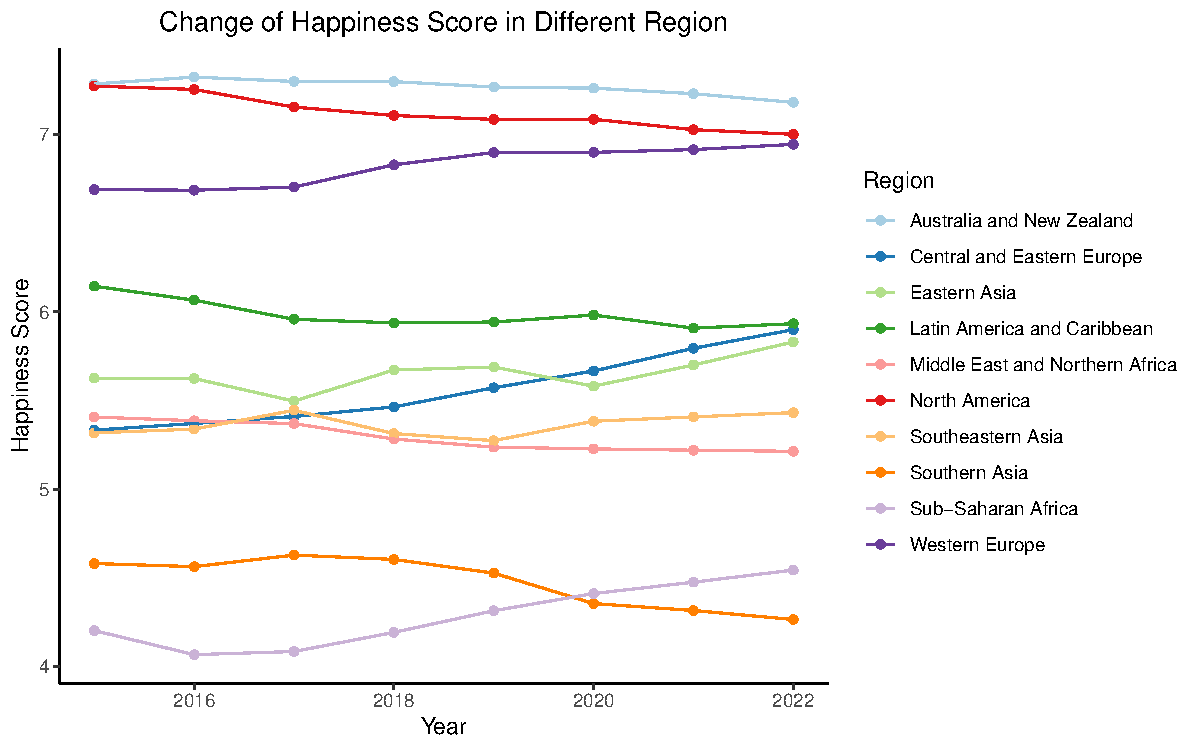
\includegraphics{Assignment4_files/figure-latex/trends -1.pdf}
\caption{(\#fig:trends )Change of Happiness Score in Different Region}
\end{figure}

From the Figure \ref{fig:trends}, we can see that the trend in all regions can be divided into three different levels of happiness score. In all regions , South Asia and Sub-Saharan Africa these two regions of overall happiness is the lowest, but Sub-Saharan Africa's happiness began to increase year by year after reaching the trough in 2016,from 4.1 to 4.5; and the South Asia region began in 2017, Happiness is declining year by year from 4.7 to 4.3. The three regions with the highest overall happiness are: Australia and New Zealand; North America; and Western Europe, and the three regions have changed their happiness by little each year,nearly 7, with a relatively flat trend. The remaining regions have overall well-being in the middle, between 5 and 6.2, with Central and Eastern Europe being the only region to increase year-over-year, while the rest of the region is in a state of slightly fluctuating but generally stable trends.Overall, we observed that regions with relatively better economic levels had higher happiness indices and more stable changes, while regions with poorer economies had lower happiness indices and had larger annual trends.

\hypertarget{the-relationship-between-economic-situation-and-health-status-with-the-happiness-in-2015-2022}{%
\subsubsection{the relationship between economic situation and health status with the happiness in 2015-2022}\label{the-relationship-between-economic-situation-and-health-status-with-the-happiness-in-2015-2022}}

People's understanding of happiness is inseparable from their own living conditions, so in this report, we also studied the relationship between happiness and economic and health status.

From the figure \ref{fig:VS}, we can find that there is a positive correlation between economic status, health status and well-being from 2015 to 2022. The better the economic status and health status, the stronger the people's well-being.

From 2015 to 2022, the influence of the economic status on the happiness score is getting lower and lower, and the influence of the health on the happiness score has increased significantly. From 2017 to 2018, the influence of economic on happiness score increased slightly, while the influence of health on happiness score decreased slightly during this period.

\begin{figure}
\centering
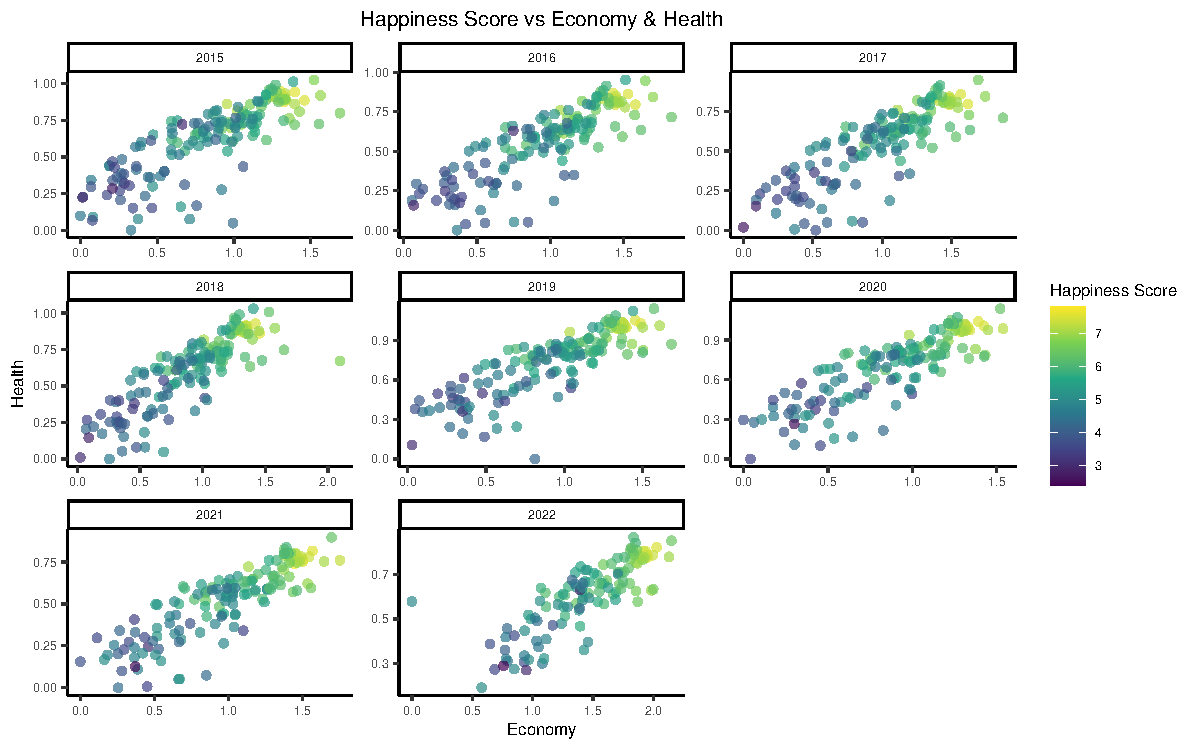
\includegraphics{Assignment4_files/figure-latex/VS -1.pdf}
\caption{(\#fig:VS )Happiness Score vs Economy \& Health}
\end{figure}

\begin{table}

\caption{\label{tab:table}A linear relationship between economic status and health status with happiness index each year}
\centering
\begin{tabular}[t]{l|r|r|r}
\hline
country & year & cases & population\\
\hline
\cellcolor{gray!6}{Afghanistan} & \cellcolor{gray!6}{1999} & \cellcolor{gray!6}{745} & \cellcolor{gray!6}{19987071}\\
\hline
Afghanistan & 2000 & 2666 & 20595360\\
\hline
\cellcolor{gray!6}{Brazil} & \cellcolor{gray!6}{1999} & \cellcolor{gray!6}{37737} & \cellcolor{gray!6}{172006362}\\
\hline
Brazil & 2000 & 80488 & 174504898\\
\hline
\cellcolor{gray!6}{China} & \cellcolor{gray!6}{1999} & \cellcolor{gray!6}{212258} & \cellcolor{gray!6}{1272915272}\\
\hline
China & 2000 & 213766 & 1280428583\\
\hline
\end{tabular}
\end{table}

Overall, from 2015 to 2022, the influence of economic on happiness score did not change significantly, in the table1 \ref{tab:table} shows the slope decreased from 1.616 to 1.406, only 0.2. However, the influence of health on happiness score changed a lot, and the slope increased from 1.2 to 2.08 Through these data, we can also see that in today's society, people pay more and more attention to their health, especially after the covid-19. Generally speaking, the proportion of health in people's mind is higher and higher.

\hypertarget{conclusions}{%
\subsubsection{Conclusions}\label{conclusions}}

Through our exploration of two research questions, we found that in economically developed countries, people's happiness is also higher, while people's happiness in economically backward areas will also be lower; and with the continuous progress of society, people's happiness comes from the impact of health, especially in the stage of covid-19. In general, some European countries and some developed countries have better welfare and medical security for their own developed economies, and people's happiness is also very high. On the contrary, in some economically poor areas, their welfare security is also poor, which also makes the happiness of the people not high.

\printbibliography

\end{document}
